\documentclass[../psets.tex]{subfiles}

\pagestyle{main}
\renewcommand{\leftmark}{Problem Set \thesection}
\setcounter{section}{4}

\begin{document}




\section{Gas-Phase Reactions II}
\subsection*{Chapter 30}
\emph{From \textcite{bib:McQuarrieSimon}.}
\begin{enumerate}[label={\textbf{30-\arabic*.}},leftmargin=3.5em]
    \setcounter{enumi}{17}
    \item \marginnote{5/18:}Consider the reaction
    \begin{equation*}
        \ce{Cl(g) + H2}(v=0) \Longrightarrow \ce{HCl($v$) + H(g)}
    \end{equation*}
    where $D_e(\ce{H2})-D_e(\ce{HCl})=\SI{12.4}{\kilo\joule\per\mole}$. Assume there is no activation barrier to the reaction. Model the reactants as hard spheres (no vibrational motion) and calculate the minimum value of the relative speed required for the reaction to occur. If we model \ce{H2(g)} and \ce{HCl(g)} as hard-sphere harmonic oscillators with $\tilde{\nu}_{\ce{H2}}=\SI{4159}{\per\centi\meter}$ and $\tilde{\nu}_{\ce{HCl}}=\SI{2886}{\per\centi\meter}$, calculate the minimum value of the relative speed required for the reaction to occur.
    \begin{proof}[Answer]
        We apply conservation of energy.
        \begin{align*}
            E_\text{reactants} &= E_\text{products}\\
            E_\text{trans}+E_\text{elec} &= E_\text{trans}'+E_\text{elec}'
        \end{align*}
        In the case that the reactants possess the \emph{minimum} energy required for a reaction to take place, there will naturally not be any excess translational energy in the products. As such, take $E_\text{trans}'=0$. Thus, making the other substitutions as dictated by the problem statement, we have that
        \begin{align*}
            \frac{1}{2}\mu u_r^2-D_e(\ce{H2}) &= 0-D_e(\ce{HCl})\\
            u_r &= \sqrt{\frac{2[D_e(\ce{H2})-D_e(\ce{HCl})](m_{\ce{H2}}+m_{\ce{HCl}})}{m_{\ce{H2}}m_{\ce{HCl}}}}\\
            &= \sqrt{\frac{2(\SI{2.06e-20}{\joule})(\SI{3.35e-27}{\kilo\gram}+\SI{5.887e-26}{\kilo\gram})}{(\SI{3.35e-27}{\kilo\gram})(\SI{5.887e-26}{\kilo\gram})}}\\
            &= \sqrt{\frac{2(\SI{2.06e-20}{\joule})(\SI{6.222e-26}{\kilo\gram})}{(\SI{3.35e-27}{\kilo\gram})(\SI{5.887e-26}{\kilo\gram})}}\\
            &= \sqrt{\SI{1.30e7}{\meter\squared\per\second\squared}}\\
            \Aboxed{u_r &= \SI[per-mode=fraction,fraction-function=\tfrac]{3606}{\meter\per\second}}
        \end{align*}
        Factoring in vibration now, we begin with a different conservation of energy statement.
        \begin{equation*}
            E_\text{trans}+E_\text{vib}+E_\text{elec} = E_\text{trans}'+E_\text{vib}'+E_\text{elec}'
        \end{equation*}
        Substituting yields
        \begin{align*}
            \frac{1}{2}\mu u_r^2+\frac{1}{2}hc\tilde{\nu}_{\ce{D2}}-D_e(\ce{H2}) &= 0+\frac{1}{2}hc\tilde{\nu}_{\ce{HCl}}-D_e(\ce{HCl})\\
            \mu u_r^2 &= hc\tilde{\nu}_{\ce{HCl}}-hc\tilde{\nu}_{\ce{D2}}+2[D_e(\ce{H2})-D_e(\ce{HCl})]\\
            u_r &= \sqrt{\frac{\{hc(\tilde{\nu}_{\ce{HCl}}-\tilde{\nu}_{\ce{D2}})+2[D_e(\ce{H2})-D_e(\ce{HCl})]\}(m_{\ce{H2}}+m_{\ce{HCl}})}{m_{\ce{H2}}m_{\ce{HCl}}}}
        \end{align*}
        so that
        \begingroup
        \allowdisplaybreaks
        \begin{align*}
            u_r &= \sqrt{\frac{\{(\num{6.626e-34})(\num{2.998e8})(\num{2.886e5}-\num{4.159e5})+2(\num{2.06e-20})\}(\num{6.222e-26})}{(\num{3.35e-27})(\num{5.887e-26})}}\\
            &= \sqrt{\frac{\{(\num{6.626e-34})(\num{2.998e8})(\num{-1.273e5})+\num{4.12e-20}\}(\num{6.222e-26})}{\num{1.97e-52}}}\\
            &= \sqrt{\frac{(\num{-2.529e-20}+\num{4.12e-20})(\num{6.222e-26})}{\num{1.97e-52}}}\\
            &= \sqrt{\frac{(\num{1.59e-20})(\num{6.222e-26})}{\num{1.97e-52}}}\\
            &= \sqrt{\num{5.02e6}}\\
            \Aboxed{u_r &= \SI[per-mode=fraction,fraction-function=\tfrac]{2241}{\meter\per\second}}
        \end{align*}
        \endgroup
    \end{proof}
    \setcounter{enumi}{21}
    \item Consider the reaction
    \begin{equation*}
        \ce{Cl(g) + HBr}(v=0) \Longrightarrow \ce{HCl($v$) + Br(g)}
    \end{equation*}
    where the relative translational energy of the reactants is \SI{9.21}{\kilo\joule\per\mole}, the difference $D_e(\ce{HBr})-D_e(\ce{HCl})=\SI{-67.2}{\kilo\joule\per\mole}$, and the activation energy for this reaction is about \SI{6}{\kilo\joule\per\mole}.\par
    Determine the range of possible vibrational states of the product molecule \ce{HCl(g)}. The spectroscopic constants for \ce{HBr(g)} and \ce{HCl(g)} are
    \begin{center}
        \begin{tabular}{ccc}
             & $\tilde{\nu}_e$ (\si{\per\centi\meter}) & $\tilde{\nu}_e\tilde{x}_e$ (\si{\per\centi\meter})\\
            \ce{HBr} & 2648.98 & 45.22\\
            \ce{HCl} & 2990.95 & 52.82\\
        \end{tabular}
    \end{center}
    Draw a diagram for this reaction that is similar to that shown in Figure 6.5 of my notes (Figure 30.8 of \textcite{bib:McQuarrieSimon}) for the \ce{F(g) + D2(g)} reaction.
    \begin{proof}[Answer]
        We have from Chapter 13 that
        \begin{equation*}
            E_\text{vib} = \tilde{\nu}_e\left( v+\frac{1}{2} \right)-\tilde{\nu}_e\tilde{x}_e\left( v+\frac{1}{2} \right)^2
        \end{equation*}
        Thus,
        \begin{align*}
            E_\text{trans}+E_\text{vib} &= E_\text{trans}+\left[ \frac{1}{2}\tilde{\nu}_e(\ce{HBr})-\frac{1}{4}\tilde{\nu}_e\tilde{x}_e(\ce{HBr}) \right]\\
            &= \SI{9.21}{\kilo\joule\per\mole}+\frac{1}{2}(\SI{31.69}{\kilo\joule\per\mole})-\frac{1}{4}(\SI{0.5409}{\kilo\joule\per\mole})\\
            &= \SI{24.92}{\kilo\joule\per\mole}
        \end{align*}
        Additionally,
        \begin{equation*}
            E_\text{elec}-E_\text{elec}' = D_e(\ce{HCl})-D_e(\ce{HBr}) = \SI{67.2}{\kilo\joule\per\mole}
        \end{equation*}
        It follows by conservation of energy that
        \begin{align*}
            E_\text{trans}+E_\text{vib}+E_\text{elec} &= E_\text{trans}'+E_\text{vib}'+E_\text{elec}'\\
            E_\text{trans}+E_\text{vib}+E_\text{elec}-E_\text{elec}' &= E_\text{trans}'+E_\text{vib}'\\
            \SI{24.92}{\kilo\joule\per\mole}+\SI{67.2}{\kilo\joule\per\mole} &= E_\text{trans}'+\left[ \tilde{\nu}_e(\ce{HCl})\left( v+\frac{1}{2} \right)-\tilde{\nu}_e\tilde{x}_e(\ce{HCl})\left( v+\frac{1}{2} \right)^2 \right]\\
            \SI{92.1}{\kilo\joule\per\mole} &\geq \left[ (\SI{35.78}{\kilo\joule\per\mole})\left( v+\frac{1}{2} \right)-(\SI{0.6319}{\kilo\joule\per\mole})\left( v+\frac{1}{2} \right)^2 \right]
        \end{align*}
        The values of $v$ that satisfy the above inequality are
        \begin{equation*}
            \boxed{v = 0,1,2}
        \end{equation*}
        The diagram is as follows.
        \begin{center}
            \begin{tikzpicture}[
                every node/.style=black
            ]
                \small
                \draw [stealth-] (0,1) -- node[rotate=90,above=8mm]{Energy (\si{\kilo\joule\per\mole})} (0,-3.8);
                \node at (3,-4.3) {Reaction coordinate};
        
                \footnotesize
                \draw
                    (0,0)    -- ++(-0.1,0) node[left]{0}
                    (0,-1.7) -- ++(-0.1,0) node[left]{-50}
                    (0,-3.4) -- ++(-0.1,0) node[left]{-100}
                ;
        
                \draw [blx,thick]
                    (0.2,0) -- node[below]{\ce{Cl + HBr}} ++(1.8,0)
                    (4,-2.3) -- node[below]{\ce{HCl + Br}} ++(1.8,0)
                ;
                \draw [blx,semithick] (2,0)
                    to[out=0,in=180,out looseness=1.3] ++(0.4,0.1)
                    to[out=0,in=180,out looseness=0.5,in looseness=0.8] ++(1.6,-2.4)
                ;
                \draw [grx,thick]
                    (0.8,0.5)  -- ++(0.6,0) node[right]{$v=0$}
                    %
                    (4.6,0.75) -- ++(0.6,0) node[right]{$v=3$}
                    (4.6,-0.1) -- ++(0.6,0) node[right]{$v=2$}
                    (4.6,-0.95) -- ++(0.6,0) node[right]{$v=1$}
                    (4.6,-1.8) -- ++(0.6,0) node[right]{$v=0$}
                ;
        
                \draw [dashed] (0.2,-2.3) -- ++(3.8,0);
                \draw [<->,shorten <=1pt,shorten >=1pt] (1.9,0) -- node[fill=white]{\SI{-67.2}{\kilo\joule\per\mole}} ++(0,-2.3);
                \draw [<->,shorten <=1pt,shorten >=1pt] (1.1,0) -- node[left]{$\frac{1}{2}h\nu_{\ce{HBr}}$} ++(0,0.5);
                %
                \draw [<->,shorten <=1pt,shorten >=1pt] (4.9,-1.8) -- node[left]{$h\nu_{\ce{HCl}}$} ++(0,0.85);
                \draw [<->,shorten <=1pt,shorten >=1pt] (4.9,-2.3) -- node[left]{$\frac{1}{2}h\nu_{\ce{HCl}}$} ++(0,0.5);
            \end{tikzpicture}
        \end{center}
    \end{proof}
    \setcounter{enumi}{30}
    \item Consider the product velocity distribution for the reaction between \ce{K(g)} and $\ce{I2}(v=0)$ at a relative translational energy of \SI{15.13}{\kilo\joule\per\mole} shown in Figure 30.13. Assume that the vibrational motion of \ce{I2(g)} and \ce{KI(g)} is harmonic with $\tilde{\nu}_{\ce{I2}}=\SI{213}{\per\centi\meter}$ and $\tilde{\nu}_{\ce{KI}}=\SI{185}{\per\centi\meter}$. Given that $D_e(\ce{I2})-D_e(\ce{KI})=\SI{-171}{\kilo\joule\per\mole}$, determine the maximum vibrational quantum number for the product \ce{KI(g)}. Now determine the speed of a $\ce{KI}(v=0)$ molecule relative to the center of mass. Repeat the calculation for the $\ce{KI}(v=1)$ molecule. Do the data in the contour map support a conclusion that \ce{KI(g)} is produced in a distribution of vibrational levels?
    \begin{proof}[Answer]
        We have that
        \begin{equation*}
            E_\text{vib} = \frac{1}{2}hc\tilde{\nu}_{\ce{I2}}
            = \frac{1}{2}\left( \frac{\SI{1}{\kilo\joule}}{\SI{e3}{\joule}} \right)(\NA\,\si{\per\mole})(\SI{6.626e-34}{\joule\second})(\SI{2.998e8}{\meter\per\second})(\SI{21300}{\per\meter})
            = \SI{1.27}{\kilo\joule\per\mole}
        \end{equation*}
        Thus, by the conservation of energy,
        \begin{align*}
            E_\text{trans}+E_\text{vib}+E_\text{elec} &= E_\text{trans}'+E_\text{vib}'+E_\text{elec}'\\
            \SI{15.13}{\kilo\joule\per\mole}+\SI{1.27}{\kilo\joule\per\mole}-D_e(\ce{I2}) &= E_\text{trans}'+E_\text{vib}'-D_e(\ce{KI})\\
            \SI{187}{\kilo\joule\per\mole}-E_\text{vib}' &= E_\text{trans}'
        \end{align*}
        All that's left is to find $v\in\N$ such that $E_\text{trans}'=187-E_\text{vib}'(v)$ is the smallest possible positive number. Since
        \begin{align*}
            E_\text{vib}' &= \left( v+\frac{1}{2} \right)hc\tilde{\nu}_{\ce{KI}}\\
            &= \left( v+\frac{1}{2} \right)\left( \frac{\SI{1}{\kilo\joule}}{\SI{e3}{\joule}} \right)(\NA\,\si{\per\mole})(\SI{6.626e-34}{\joule\second})(\SI{2.998e8}{\meter\per\second})(\SI{18500}{\per\meter})\\
            &= (\SI{2.21}{\kilo\joule\per\mole})\left( v+\frac{1}{2} \right)
        \end{align*}
        we have that
        \begin{align*}
            E_\text{vib}' &= \SI{187}{\kilo\joule\per\mole}\\
            (\SI{2.22}{\kilo\joule\per\mole})\left( v+\frac{1}{2} \right) &= \SI{187}{\kilo\joule\per\mole}\\
            v &= 84.1
        \end{align*}
        Therefore, the maximum vibrational quantum number for the product \ce{KI(g)} is
        \begin{equation*}
            \boxed{v = 84}
        \end{equation*}
        To determine the speed of a $\ce{KI}(v=0)$ molecule, we may perform the following calculation.
        \begin{align*}
            E_\text{trans}' &= \SI{187}{\kilo\joule\per\mole}-E_\text{vib}'\\
            \frac{1}{2}\mu'{u_r'}^2 &= \SI{187}{\kilo\joule\per\mole}-(\SI{2.21}{\kilo\joule\per\mole})\left( 0+\frac{1}{2} \right)\\
            \frac{m_{\ce{KI}}m_{\ce{I}}}{2(m_{\ce{KI}}+m_{\ce{I}})}{u_r'}^2 &= \SI{187}{\kilo\joule\per\mole}-\SI{1.11}{\kilo\joule\per\mole}\\
            u_r' &= \sqrt{\frac{(\SI{186}{\kilo\joule\per\mole})(2)(\SI{2.757e-25}{\kilo\gram}+\SI{2.107e-25}{\kilo\gram})}{(\SI{2.757e-25}{\kilo\gram})(\SI{2.107e-25}{\kilo\gram})}}\\
            &= \sqrt{\frac{(\SI{3.09e-19}{\joule})(2)(\SI{4.864e-25}{\kilo\gram})}{(\SI{2.757e-25}{\kilo\gram})(\SI{2.107e-25}{\kilo\gram})}}\\
            &= \sqrt{\SI{5.17e6}{\meter\squared\per\second\squared}}\\
            \Aboxed{u_r' &= \SI[per-mode=fraction,fraction-function=\tfrac]{2274}{\meter\per\second}}
        \end{align*}
        For a $\ce{KI}(v=1)$ molecule, we perform an analogous calculation.
        \begin{align*}
            E_\text{trans}' &= \SI{187}{\kilo\joule\per\mole}-E_\text{vib}'\\
            \frac{1}{2}\mu'{u_r'}^2 &= \SI{187}{\kilo\joule\per\mole}-(\SI{2.21}{\kilo\joule\per\mole})\left( 1+\frac{1}{2} \right)\\
            \frac{m_{\ce{KI}}m_{\ce{I}}}{2(m_{\ce{KI}}+m_{\ce{I}})}{u_r'}^2 &= \SI{187}{\kilo\joule\per\mole}-\SI{3.32}{\kilo\joule\per\mole}\\
            u_r' &= \sqrt{\frac{(\SI{184}{\kilo\joule\per\mole})(2)(\SI{2.757e-25}{\kilo\gram}+\SI{2.107e-25}{\kilo\gram})}{(\SI{2.757e-25}{\kilo\gram})(\SI{2.107e-25}{\kilo\gram})}}\\
            &= \sqrt{\frac{(\SI{3.06e-19}{\joule})(2)(\SI{4.864e-25}{\kilo\gram})}{(\SI{2.757e-25}{\kilo\gram})(\SI{2.107e-25}{\kilo\gram})}}\\
            &= \sqrt{\SI{5.12e6}{\meter\squared\per\second\squared}}\\
            \Aboxed{u_r' &= \SI[per-mode=fraction,fraction-function=\tfrac]{2264}{\meter\per\second}}
        \end{align*}
        \fbox{Yes} the data in the contour map supports the conclusion that \ce{KI(g)} is produced in a distribution of vibrational levels since there is such significant spread in observed speeds.
    \end{proof}
    \setcounter{enumi}{43}
    \item Below is a drawing of the contour plot of the potential-energy surface of the collinear \ce{H(g) + H2(g)} reaction in the vicinity of the transition state. We take $r_{12}$ and $r_{23}$ to be the bond length of the \ce{H2} reactant and product, respectively. Label the location of the transition state. Draw a dashed line that indicates the lowest energy path for the reaction. Draw a two-dimensional representation of the reaction path in which you plot $V(r_{12},r_{23})$ as a function of $r_{12}-r_{23}$.
    \begin{center}
        % \includegraphics[width=0.345\linewidth]{contours.png}
        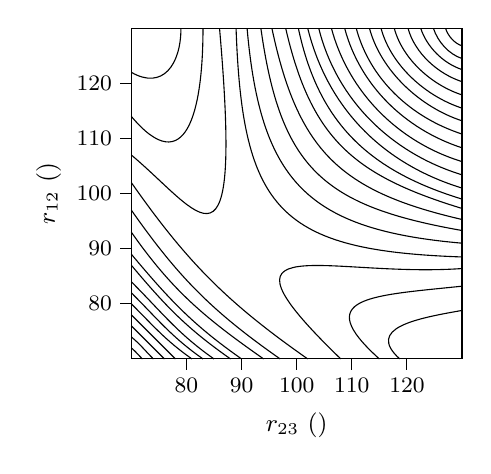
\begin{tikzpicture}[
            % remember picture,overlay,
            % xshift=-4.47cm,yshift=1.08cm,
            % xscale=0.7,yscale=0.73
            scale=0.7
        ]
            \draw (0,0) rectangle (6,6);
    
            \small
            \node at (3,-1.2) {$r_{23}$ (\si{\pico\meter})};
            \node [rotate=90] at (-1.5,3) {$r_{12}$ (\si{\pico\meter})};
    
            \footnotesize
            \draw
                (1,0) -- ++(0,-0.2) node[below]{80}
                (2,0) -- ++(0,-0.2) node[below]{90}
                (3,0) -- ++(0,-0.2) node[below]{100}
                (4,0) -- ++(0,-0.2) node[below]{110}
                (5,0) -- ++(0,-0.2) node[below]{120}
            ;
            \draw
                (0,1) -- ++(-0.2,0) node[left]{80}
                (0,2) -- ++(-0.2,0) node[left]{90}
                (0,3) -- ++(-0.2,0) node[left]{100}
                (0,4) -- ++(-0.2,0) node[left]{110}
                (0,5) -- ++(-0.2,0) node[left]{120}
            ;
    
            \draw
                (0,5.2) to[out=-30,in=-90,looseness=1.4] (0.9,6)
                (0,4.4) to[out=-50,in=-90,looseness=1.9] (1.3,6)
                (0,3.7) to[out=-40,in=-85,out looseness=1.5,in looseness=4.4] (1.6,6)
                %
                (0,3.2) to[out=-55,in=145] (3.2,0)
                (0,2.7) to[out=-55,in=145] (2.7,0)
                (0,2.3) to[out=-55,in=145] (2.4,0)
                (0,1.9) to[out=-50,in=145] (2.0,0)
                (0,1.7) to[out=-50,in=145] (1.8,0)
                (0,1.4) to[out=-45,in=145] (1.5,0)
                (0,1.2) to[out=-45,in=145] (1.3,0)
                (0,1.0) to[out=-45,in=145] (1.1,0)
                (0,0.8) to[out=-45,in=135] (0.8,0)
                (0,0.6) to[out=-45,in=135] (0.6,0)
                (0,0.4) to[out=-40,in=135] (0.4,0)
                (0,0.2) to[out=-40,in=135] (0.2,0)
                %
                (1.90,6) to[out=-88,in=178,looseness=1.45] (6,1.85)
                (2.10,6) to[out=-85,in=175,looseness=1.30] (6,2.1)
                (2.35,6) to[out=-82,in=170,looseness=1.27] (6,2.33)
                (2.55,6) to[out=-78,in=167,looseness=1.19] (6,2.53)
                (2.80,6) to[out=-77,in=163,looseness=1.15] (6,2.73)
                (3.03,6) to[out=-78,in=163,looseness=1.05] (6,2.9)
                (3.20,6) to[out=-76,in=163,looseness=0.95] (6,3.1)
                (3.40,6) to[out=-76,in=163,looseness=0.92] (6,3.34)
                (3.63,6) to[out=-75,in=163,looseness=0.91] (6,3.58)
                (3.87,6) to[out=-75,in=162,looseness=0.91] (6,3.83)
                (4.08,6) to[out=-75,in=162,looseness=0.91] (6,4.08)
                (4.32,6) to[out=-75,in=162,looseness=0.86] (6,4.32)
                (4.53,6) to[out=-75,in=162,looseness=0.86] (6,4.55)
                (4.77,6) to[out=-75,in=162,looseness=0.86] (6,4.79)
                (5.02,6) to[out=-75,in=162,looseness=0.86] (6,5.03)
                (5.25,6) to[out=-72,in=162,looseness=0.86] (6,5.25)
                (5.48,6) to[out=-72,in=162,looseness=0.86] (6,5.45)
                (5.70,6) to[out=-72,in=162,looseness=0.86] (6,5.68)
                %
                (3.80,0) to[out=136,in=-176,out looseness=3.3,in looseness=2.3] (6,1.64)
                (4.50,0) to[out=138,in=-174,looseness=2.15] (6,1.32)
                (4.87,0) to[out=138,in=-170,looseness=1.5] (6,0.88)
            ;
        \end{tikzpicture}
    \end{center}
    \begin{proof}[Answer]
        ${\color{white}hi}$
        \begin{figure}[H]
            \centering
            \begin{subfigure}[b]{0.49\linewidth}
                \centering
                \begin{tikzpicture}[scale=0.7]
                    \draw (0,0) rectangle (6,6);
            
                    \small
                    \node at (3,-1.2) {$r_{23}$ (\si{\pico\meter})};
                    \node [rotate=90] at (-1.5,3) {$r_{12}$ (\si{\pico\meter})};
            
                    \footnotesize
                    \draw
                        (1,0) -- ++(0,-0.2) node[below]{80}
                        (2,0) -- ++(0,-0.2) node[below]{90}
                        (3,0) -- ++(0,-0.2) node[below]{100}
                        (4,0) -- ++(0,-0.2) node[below]{110}
                        (5,0) -- ++(0,-0.2) node[below]{120}
                    ;
                    \draw
                        (0,1) -- ++(-0.2,0) node[left]{80}
                        (0,2) -- ++(-0.2,0) node[left]{90}
                        (0,3) -- ++(-0.2,0) node[left]{100}
                        (0,4) -- ++(-0.2,0) node[left]{110}
                        (0,5) -- ++(-0.2,0) node[left]{120}
                    ;
            
                    \draw
                        (0,5.2) to[out=-30,in=-90,looseness=1.4] (0.9,6)
                        (0,4.4) to[out=-50,in=-90,looseness=1.9] (1.3,6)
                        (0,3.7) to[out=-40,in=-85,out looseness=1.5,in looseness=4.4] (1.6,6)
                        %
                        (0,3.2) to[out=-55,in=145] (3.2,0)
                        (0,2.7) to[out=-55,in=145] (2.7,0)
                        (0,2.3) to[out=-55,in=145] (2.4,0)
                        (0,1.9) to[out=-50,in=145] (2.0,0)
                        (0,1.7) to[out=-50,in=145] (1.8,0)
                        (0,1.4) to[out=-45,in=145] (1.5,0)
                        (0,1.2) to[out=-45,in=145] (1.3,0)
                        (0,1.0) to[out=-45,in=145] (1.1,0)
                        (0,0.8) to[out=-45,in=135] (0.8,0)
                        (0,0.6) to[out=-45,in=135] (0.6,0)
                        (0,0.4) to[out=-40,in=135] (0.4,0)
                        (0,0.2) to[out=-40,in=135] (0.2,0)
                        %
                        (1.90,6) to[out=-88,in=178,looseness=1.45] (6,1.85)
                        (2.10,6) to[out=-85,in=175,looseness=1.30] (6,2.1)
                        (2.35,6) to[out=-82,in=170,looseness=1.27] (6,2.33)
                        (2.55,6) to[out=-78,in=167,looseness=1.19] (6,2.53)
                        (2.80,6) to[out=-77,in=163,looseness=1.15] (6,2.73)
                        (3.03,6) to[out=-78,in=163,looseness=1.05] (6,2.9)
                        (3.20,6) to[out=-76,in=163,looseness=0.95] (6,3.1)
                        (3.40,6) to[out=-76,in=163,looseness=0.92] (6,3.34)
                        (3.63,6) to[out=-75,in=163,looseness=0.91] (6,3.58)
                        (3.87,6) to[out=-75,in=162,looseness=0.91] (6,3.83)
                        (4.08,6) to[out=-75,in=162,looseness=0.91] (6,4.08)
                        (4.32,6) to[out=-75,in=162,looseness=0.86] (6,4.32)
                        (4.53,6) to[out=-75,in=162,looseness=0.86] (6,4.55)
                        (4.77,6) to[out=-75,in=162,looseness=0.86] (6,4.79)
                        (5.02,6) to[out=-75,in=162,looseness=0.86] (6,5.03)
                        (5.25,6) to[out=-72,in=162,looseness=0.86] (6,5.25)
                        (5.48,6) to[out=-72,in=162,looseness=0.86] (6,5.45)
                        (5.70,6) to[out=-72,in=162,looseness=0.86] (6,5.68)
                        %
                        (3.80,0) to[out=136,in=-176,out looseness=3.3,in looseness=2.3] (6,1.64)
                        (4.50,0) to[out=138,in=-174,looseness=2.15] (6,1.32)
                        (4.87,0) to[out=138,in=-170,looseness=1.5] (6,0.88)
                    ;
            
                    \draw [rex,thick,dashed] (6,0) to[out=160,in=-80,looseness=1.2] (0.3,6);
                    \fill [rex] (2,2.1) circle (3pt) node[above right]{TS};
                \end{tikzpicture}
            \end{subfigure}
            \begin{subfigure}[b]{0.49\linewidth}
                \centering
                \begin{tikzpicture}
                    \small
                    \draw [stealth-stealth] (-3,0) -- node[below]{$r_{12}-r_{23}$} (3,0);
                    \draw [-stealth] (0,0) -- ++(0,2) node[above]{$V$};
                    
                    \draw [rex,thick]
                        plot[domain=-2.9:-0.001] (\x,{1/(1+\x*\x)})
                        plot[domain=0.001:2.9] (\x,{1/(1+\x*\x)})
                    ;
                \end{tikzpicture}
            \end{subfigure}
        \end{figure}
    \end{proof}
\end{enumerate}


\subsection*{Application}
\begin{enumerate}[label={\arabic*)}]
    \item Name one HW problem you would like to develop into a thought experiment or relate to a literature article.
    \item Describe how the idea or conclusion from the HW problem applies to the research idea in 1-2 paragraphs (word limit: 300). Once again, this can either be a thought experiment or an experiment found in the literature.
    \item You do not need to derive any equations in this short discussion. Use your intuition and focus on the big picture.
    \item Please cite the literature if you link the HW problem to anyone (author names, titles, journal name, volume numbers, and page numbers).
\end{enumerate}
\begin{proof}[Answer]
    I would like to relate Problem 30-44 to the principle of microscopic reversibility. Earlier this quarter, I was introduced to the principle of microscopic reversibility in Organic Chemistry III. Essentially, this postulate asserts that for reversible reactions, the mechanism of the reverse reaction is the stepwise inverse of the mechanism of the forward reaction. Although this made some sense at the time, largely due to my professor's justification of it as "a reaction will always proceed by the lowest energy path, and what's lowest energy forward will naturally be lowest energy in reverse," I failed to fully grasp the sentiment until today.\par
    In this problem, we are asked to trace what is essentially a potential energy "canyon." Now our reactants can move anywhere in the canyon, including climbing up the walls, but they will be more likely to climb the small hills and stay where the ground is relatively low, following that path. Another thing to note is that if the reactants (now products) decide to migrate back towards where they started, the easiest way to do so will naturally be the way they came (along the canyon floor). To me, this potential energy surface picture makes the principle of microscopic reversibility appear not just semi-logical, but inevitable.
\end{proof}




\end{document}